% Prácticas de laboratorio de cada unidad.
% Se incluye en el anexo de Libro_4_ESO_ES.tex. Ordenado por unidades.

%========================================================================================
\section[Unidad 1. Comprobación de una hipótesis]{Unidad 1. Comprobación de una hipótesis científica}
%========================================================================================
% (sacado del final de UD1_Trabajo_cientifico.tex)

La \textbf{velocidad de una reacción química} es la cantidad de sustancia que se forma o se transforma por unidad de tiempo. El carbonato de calcio reacciona con el ácido clorhídrico y desprende dióxido de carbono:
\[ \ch{CaCO3 (s) + 2 HCl (aq) -> CaCl2 (aq) + CO2 (g) + H2O (l)} \]
\textbf{Hipótesis:} la superficie de contacto influye en la velocidad de la reacción: esta es mayor cuando el carbonato de calcio está pulverizado que cuando está en fragmentos.

\begin{figure}[H]
    \centering
    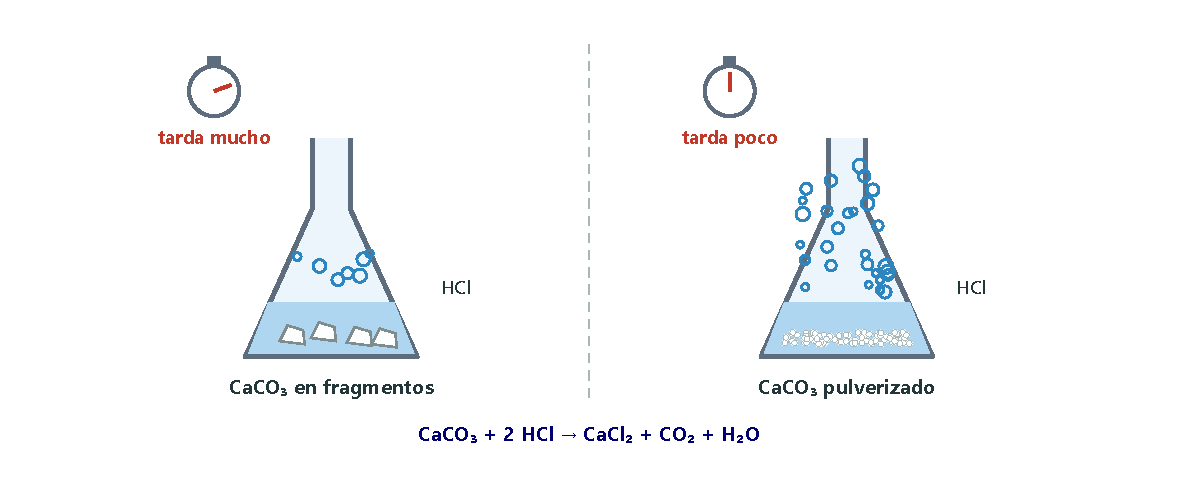
\includegraphics[width=0.8\textwidth]{images/UD1/practica_superficie}
    \caption{Reacción del carbonato de calcio en fragmentos y pulverizado con ácido clorhídrico.}
    \label{fig:practica_superficie}
\end{figure}

\noindent\begin{minipage}[t]{0.5\textwidth}
    \textbf{Objetivos}
    \begin{itemize}
        \item Comprobar una hipótesis mediante la experimentación.
        \item Medir masas, volúmenes y tiempos.
        \item Trabajar con seguridad en el laboratorio.
    \end{itemize}
\end{minipage}\hfill
\begin{minipage}[t]{0.46\textwidth}
    \textbf{Material}
    \begin{itemize}
        \item Balanza, probeta, dos Erlenmeyer y dos vidrios de reloj.
        \item Carbonato de calcio y ácido clorhídrico diluido.
        \item Un cronómetro.
    \end{itemize}
\end{minipage}

\medskip

\textbf{Procedimiento}
\begin{enumerate}[label=\numberballgreen]
    \item Pesa dos muestras iguales de carbonato de calcio: una en fragmentos y otra pulverizada.
    \item Pon el carbonato en fragmentos en un Erlenmeyer, añade un volumen medido de ácido clorhídrico y pon en marcha el cronómetro. Detenlo cuando desaparezca todo el sólido.
    \item Repite la experiencia con el carbonato pulverizado, la misma cantidad de ácido y el mismo cronómetro.
\end{enumerate}

\begin{exercise}
    Responde a estas preguntas sobre la práctica:
    \begin{enumerate}[label=\alph*)]
        \item ¿Cuál es la variable independiente? ¿Y la dependiente? ¿Qué variables deben estar controladas?
        \item ¿Por qué es importante usar el mismo cronómetro y la misma cantidad de ácido?
        \item Un grupo obtiene \qty{185}{\s} con los fragmentos y \qty{40}{\s} con el polvo. ¿Se confirma la hipótesis? ¿Cuántas veces más rápida ha sido la reacción con el polvo?
    \end{enumerate}
    \begin{solu}
        a) Independiente: el \textcolor{red}{grado de división} del sólido (superficie de contacto). Dependiente: el \textcolor{red}{tiempo} que tarda en desaparecer. Controladas: la \textcolor{red}{masa} de carbonato, el \textcolor{red}{volumen y la concentración} del ácido, la temperatura\ldots
        b) Para que solo cambie la variable que estudiamos y las medidas sean \textcolor{red}{comparables}.
        c) \textcolor{red}{Sí}: con el polvo la reacción termina antes. Es \(\dfrac{185}{40} = \textcolor{red}{\num{4.6}}\) veces más rápida.
    \end{solu}
\end{exercise}

%========================================================================================
\section{Unidad 2. Propiedades de los elementos}
%========================================================================================
% (sacado del final de UD_2_el_atomo_tp.tex)

Vamos a comprobar experimentalmente algunas propiedades que distinguen a los metales de los no metales, usando tres metales (cobre, aluminio y zinc) y un no metal (carbono en forma de grafito, la mina de un lápiz).

\begin{multicols}{2}
    \textbf{Objetivos}
    \begin{itemize}
        \item Manejar materiales e instrumentos del laboratorio de Química.
        \item Respetar las normas de seguridad.
        \item Comprobar la conductividad, la solubilidad en agua y la reacción con ácido clorhídrico de varios elementos.
    \end{itemize}
    \columnbreak
    \textbf{Material}
    \begin{itemize}
        \item Cobre, aluminio, zinc y grafito.
        \item Un circuito sencillo (pila, cables y bombilla o LED).
        \item Ácido clorhídrico diluido (\ch{HCl}), agua.
        \item Vaso de precipitados y tubos de ensayo.
    \end{itemize}
\end{multicols}

\textbf{Procedimiento}
\begin{enumerate}[label=\numberballgreen]
    \item Observa el aspecto de cada elemento (¿tiene brillo metálico?).
    \item Echa un poco de cada uno en un tubo de ensayo con agua y comprueba si se disuelve.
    \item Pon un trozo de zinc en un tubo con unos mililitros de ácido clorhídrico y observa si hay reacción (burbujas). Repite con los demás elementos. \textbf{Usa gafas y guantes.}
    \item Intercala cada elemento en el circuito y comprueba si la bombilla se enciende.
\end{enumerate}

\begin{exercise}
    Recoge tus resultados en una tabla con las columnas: elemento, aspecto, densidad, solubilidad en agua, reacción con \ch{HCl} y conductividad eléctrica (busca las densidades en Internet). ¿Conduce el grafito la corriente? ¿Es eso habitual en los no metales? ¿Qué gas se desprende cuando el ácido reacciona con el zinc y el aluminio? ¿Cómo medirías la densidad de cada elemento en el laboratorio?
    \begin{solu}
        \begin{center}
            % --- tabla antigua ---
            % \begin{tblr}{colspec={lccccc}, hlines, vlines, row{1}={font=\bfseries}}
                % Elemento & Aspecto & Densidad (\unit{\gram\per\cubic\centi\metre}) & Solubilidad & Con \ch{HCl} & Conduce \\
                % Aluminio & metálico & \num{2.70} & insoluble & desprende \ch{H2} & sí \\
                % Grafito & no metálico & \num{2.26} & insoluble & no reacciona & sí \\
                % Zinc & metálico & \num{7.14} & insoluble & desprende \ch{H2} & sí \\
                % Cobre & metálico & \num{8.96} & insoluble & no reacciona & sí \\
            % \end{tblr}
            % --- tabla nueva ---
            \begin{tabular}{@{}lccccc@{}}
                \toprule
                \textbf{Elemento} & \textbf{Aspecto} & \textbf{Densidad (\unit{\gram\per\cubic\centi\metre})} & \textbf{Solubilidad} & \textbf{Con \ch{HCl}} & \textbf{Conduce} \\
                \midrule
                Aluminio & metálico & \num{2.70} & insoluble & desprende \ch{H2} & sí \\[3pt]
                Grafito & no metálico & \num{2.26} & insoluble & no reacciona & sí \\[3pt]
                Zinc & metálico & \num{7.14} & insoluble & desprende \ch{H2} & sí \\[3pt]
                Cobre & metálico & \num{8.96} & insoluble & no reacciona & sí \\
                \bottomrule
            \end{tabular}
        \end{center}
        El grafito conduce la corriente, pero es una excepción: los no metales, en general, no conducen. El gas desprendido es \textcolor{red}{hidrógeno}, \ch{H2}. La densidad se calcula midiendo la masa con una balanza y el volumen por desplazamiento de agua en una probeta: \(d = m/V\).
    \end{solu}
\end{exercise}

%========================================================================================
\section{Unidad 3. Propiedades de las sustancias y enlace químico}
%========================================================================================
% (sacado del final de UD3_enlace_quimico.tex)

Vamos a estudiar algunas propiedades del sulfato de cobre(II), \ch{CuSO4}, el cloruro de potasio, \ch{KCl}, y el dióxido de silicio, \ch{SiO2} (arena fina), en estado sólido y en disolución. A partir de los resultados deduciremos qué tipo de enlace tiene cada sustancia.

\begin{multicols}{2}
    \textbf{Objetivos}
    \begin{itemize}
        \item Manejar materiales e instrumentos del laboratorio de Química.
        \item Respetar las normas de seguridad.
        \item Valorar la importancia del trabajo experimental sistemático.
        \item Comprobar la dureza, la solubilidad y la conductividad eléctrica de varias sustancias.
    \end{itemize}
    \columnbreak
    \textbf{Material}
    \begin{itemize}
        \item \ch{CuSO4}, \ch{KCl} y \ch{SiO2}; un clavo.
        \item Agua destilada, tetracloruro de carbono (\ch{CCl4}), seis tubos de ensayo y una gradilla.
        \item Pila de \qty{9}{\volt} o \qty{12}{\volt}, cables con pinzas de cocodrilo, bombilla o LED, dos electrodos, cápsula de porcelana y vaso de precipitados.
    \end{itemize}
\end{multicols}

\textbf{Procedimiento}
\begin{enumerate}[label=\numberballgreen]
    \item \textbf{Dureza.} Intenta rayar cada sustancia con la punta de un clavo y anota lo que observas.
    \item \textbf{Solubilidad en agua} (disolvente polar). Pon un poco de cada sustancia en un tubo de ensayo, añade agua destilada hasta la mitad y agita. Anota cuáles se disuelven.
    \item \textbf{Solubilidad en tetracloruro de carbono} (disolvente apolar). Repite el paso anterior con \ch{CCl4} (hasta un tercio del tubo). \textbf{Hazlo en la vitrina de gases, con gafas y guantes.}
    \item \textbf{Conductividad del sólido.} Coloca cada sólido en la cápsula de porcelana, introduce los electrodos y comprueba si se enciende la bombilla.
    \item \textbf{Conductividad de la disolución.} Repite la prueba con las disoluciones acuosas de las sustancias que se hayan disuelto.
\end{enumerate}

\begin{exercise}
    Recoge tus resultados en una tabla con las columnas: dureza, solubilidad en agua, solubilidad en \ch{CCl4}, conductividad en estado sólido y conductividad en disolución acuosa, para el \ch{CuSO4}, el \ch{KCl} y el \ch{SiO2}.
    \begin{solu}
        Respuesta según los resultados del laboratorio. Lo esperable es:
        \begin{center}
            % --- tabla antigua ---
            % \begin{tblr}{colspec={lccccc}, hlines, vlines, row{1}={font=\bfseries}}
                % & Dureza & Agua & \ch{CCl4} & Sólido & Disolución \\
                % \ch{CuSO4} & duro, frágil & soluble & insoluble & no conduce & conduce \\
                % \ch{KCl} & duro, frágil & soluble & insoluble & no conduce & conduce \\
                % \ch{SiO2} & muy duro & insoluble & insoluble & no conduce & --- \\
            % \end{tblr}
            % --- tabla nueva ---
            \begin{tabular}{@{}lccccc@{}}
                \toprule
                 & \textbf{Dureza} & \textbf{Agua} & \textbf{\ch{CCl4}} & \textbf{Sólido} & \textbf{Disolución} \\
                \midrule
                \ch{CuSO4} & duro, frágil & soluble & insoluble & no conduce & conduce \\[3pt]
                \ch{KCl} & duro, frágil & soluble & insoluble & no conduce & conduce \\[3pt]
                \ch{SiO2} & muy duro & insoluble & insoluble & no conduce & --- \\
                \bottomrule
            \end{tabular}
        \end{center}
    \end{solu}
\end{exercise}

\begin{exercise}
    A partir de tus resultados, ¿qué tipo de enlace tiene cada sustancia? ¿Qué propiedades físicas y químicas presentan?
    \begin{solu}
        \textcolor{red}{\ch{CuSO4}: iónico} (entre el catión \ch{Cu^{2+}} y el anión \ch{SO4^{2-}}). Es soluble en agua y no conduce en estado sólido, pero sí disuelto.
        \textcolor{red}{\ch{KCl}: iónico} (entre \ch{K+} y \ch{Cl-}). Mismo comportamiento: soluble en agua y conductor solo en disolución.
        \textcolor{red}{\ch{SiO2}: covalente reticular}. Es muy duro, insoluble en agua y en \ch{CCl4} y no conduce la corriente.
    \end{solu}
\end{exercise}

%========================================================================================
\section[Unidad 4. Carbono en un compuesto]{Unidad 4. Investigación de la existencia de carbono en un compuesto}
%========================================================================================
% (sacado del final de UD4_organica.tex)

Vamos a comprobar si una sustancia contiene carbono. Al calentarla con óxido de cobre(II), el carbono se oxida a dióxido de carbono, \ch{CO2}. Si este gas se hace burbujear en una disolución de hidróxido de calcio (agua de cal), se forma carbonato de calcio, \ch{CaCO3}, un sólido blanco insoluble en agua (es el componente principal de la roca caliza):
\[ \ch{Ca(OH)2 (aq) + CO2 (g) -> CaCO3 (s) + H2O (l)} \]

\begin{figure}[H]
    \centering
    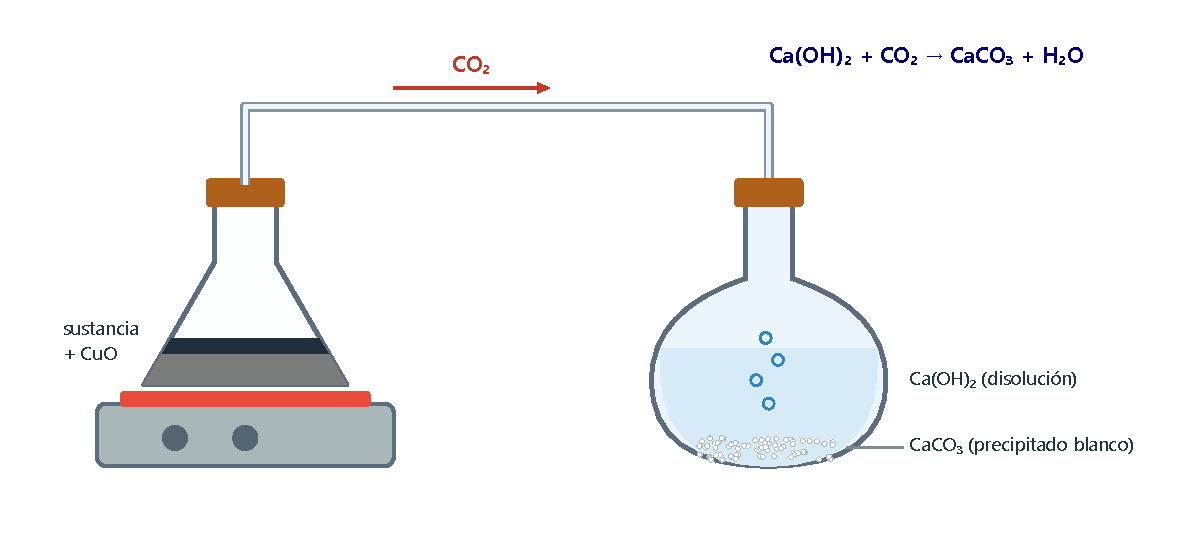
\includegraphics[width=0.9\textwidth]{images/UD4/practica_carbono}
    \caption{Montaje para detectar el carbono de un compuesto.}
    \label{fig:practica_carbono}
\end{figure}

\noindent\begin{minipage}[t]{0.48\textwidth}
    \textbf{Objetivos}
    \begin{itemize}
        \item Detectar la presencia de carbono en un compuesto.
        \item Trabajar con materiales e instrumentos del laboratorio.
        \item Respetar las normas de seguridad al manejar sustancias peligrosas.
    \end{itemize}
\end{minipage}\hfill
\begin{minipage}[t]{0.48\textwidth}
    \textbf{Material}
    \begin{itemize}
        \item Un matraz Erlenmeyer y un matraz aforado, con tapones horadados.
        \item Una placa calefactora y un tubo de vidrio en doble L.
        \item Hidróxido de calcio y óxido de cobre(II).
        \item Una sustancia con carbono (azúcar, almidón\ldots).
    \end{itemize}
\end{minipage}

\medskip

\textbf{Procedimiento}
\begin{enumerate}[label=\numberballgreen]
    \item Pon en el Erlenmeyer una mezcla de la sustancia con aproximadamente el triple de óxido de cobre(II) en polvo, previamente calcinado, y cubre la mezcla con más óxido de cobre.
    \item Cierra el Erlenmeyer con el tapón y el tubo de desprendimiento en doble L.
    \item Introduce el otro extremo del tubo en una disolución de hidróxido de calcio contenida en el matraz aforado, cerrado con el otro tapón (figura~\ref{fig:practica_carbono}).
    \item Calienta la mezcla para que los gases que se desprenden burbujeen en la disolución.
\end{enumerate}

\begin{exercise}
    Responde a estas preguntas sobre la práctica:
    \begin{enumerate}[label=\alph*)]
        \item Describe lo que sucede en el matraz aforado. ¿Qué significa?
        \item ¿Qué confirma que la sustancia de partida contiene carbono?
        \item ¿De dónde procede el \ch{CO2}? ¿Qué le ocurre al \ch{CaCO3}?
        \item ¿Qué sucedería si soplaras a través de un tubo sumergido en la disolución de hidróxido de calcio? ¿Por qué?
    \end{enumerate}
    \begin{solu}
        a) Se desprenden burbujas de un gas y la disolución \textcolor{red}{se enturbia}: se ha formado un sólido blanco. Significa que se ha desprendido \ch{CO2}.
        b) La formación del \textcolor{red}{precipitado blanco de carbonato de calcio}.
        c) El \ch{CO2} procede de la reacción del \textcolor{red}{carbono de la sustancia con el óxido de cobre(II)}, que aporta el oxígeno. El \ch{CaCO3} es insoluble y \textcolor{red}{precipita}.
        d) También se \textcolor{red}{enturbiaría}, porque el aire que expulsamos contiene \ch{CO2}, procedente de la oxidación de los compuestos del carbono de los alimentos en las células.
    \end{solu}
\end{exercise}

%========================================================================================
\section{Unidad 5. Separación de una mezcla de alcohol y agua}
%========================================================================================
% (sacado del final de UD5_Sistema_materiales.tex)

El alcohol (etanol) y el agua tienen temperaturas de ebullición distintas, así que podemos separarlos por \textbf{destilación} (figura~\ref{fig:separacion_disoluciones}).

\begin{multicols}{2}
    \textbf{Objetivos}
    \begin{itemize}
        \item Manejar materiales e instrumentos del laboratorio.
        \item Respetar las normas de seguridad.
        \item Valorar el trabajo experimental sistemático.
        \item Separar los componentes de una disolución de alcohol y agua.
    \end{itemize}
    \columnbreak
    \textbf{Material}
    \begin{itemize}
        \item Matraz de destilación (o matraz con cabeza de destilación) y termómetro.
        \item Placa calefactora, cristalizador (baño María), dos soportes con pinzas.
        \item Refrigerante con gomas de entrada y salida de agua.
        \item Erlenmeyer, probeta de \qty{100}{\mL}, alcohol y agua.
    \end{itemize}
\end{multicols}

\textbf{Procedimiento}
\begin{enumerate}[label=\numberballgreen]
    \item Prepara una disolución de alcohol en agua al \qty{90}{\percent} en volumen.
    \item Monta el aparato de destilación y pon la disolución en el matraz.
    \item Conecta la goma de entrada de agua a la parte baja del refrigerante y lleva la de salida al fregadero.
    \item Calienta el matraz con la placa calefactora o al baño María. \textbf{El alcohol es inflamable: nunca uses una llama.}
    \item Anota la temperatura cuando el alcohol empiece a destilar: verás que se mantiene constante.
    \item Deja de calentar cuando la temperatura empiece a subir de nuevo.
\end{enumerate}

\begin{exercise}
    Responde a estas preguntas sobre la práctica:
    \begin{enumerate}[label=\alph*)]
        \item ¿Para qué sirve el refrigerante?
        \item ¿Por qué el agua entra por la parte baja del refrigerante y sale por la alta, y no al revés?
        \item ¿Para qué sirve el termómetro? ¿Qué temperatura marca cuando el alcohol empieza a destilar?
        \item ¿Durante cuánto tiempo se mantiene constante la temperatura? ¿Qué ocurre cuando empieza a subir?
        \item ¿Qué se recoge en el Erlenmeyer y qué queda en el matraz de destilación?
    \end{enumerate}
    \begin{solu}
        a) Para \textcolor{red}{enfriar el vapor} que sale del matraz y condensarlo, de modo que se pueda recoger como líquido.
        b) Así el agua fría recorre el refrigerante en sentido contrario al vapor, el tubo se llena bien de agua y el vapor se encuentra con agua cada vez más fría a medida que avanza.
        c) Para controlar la temperatura del vapor y saber qué sustancia destila. Unos \textcolor{red}{\qty{78}{\celsius}}, la temperatura de ebullición del etanol.
        d) Mientras queda alcohol por evaporar, porque la energía se emplea en el cambio de estado. Cuando sube, \textcolor{red}{ya se ha separado todo el alcohol} y se está calentando el agua.
        e) En el Erlenmeyer, el \textcolor{red}{alcohol}; en el matraz, el \textcolor{red}{agua}.
    \end{solu}
\end{exercise}

%========================================================================================
\section{Unidad 6. Estudio de una reacción de neutralización}
%========================================================================================
% (sacado del final de UD6_reacciones_quimicas.tex)

Vamos a usar una reacción de neutralización para averiguar la concentración de una disolución de \ch{HCl} (una \textbf{valoración}) y aprenderemos a usar un pH-metro. Es un instrumento delicado: el electrodo no debe chocar con el vaso ni con el agitador, hay que lavarlo con agua destilada después de cada medida y guardarlo sumergido en agua destilada.

\begin{multicols}{2}
    \textbf{Objetivos}
    \begin{itemize}
        \item Trabajar con sustancias e instrumentos del laboratorio de Química.
        \item Respetar las normas de seguridad con sustancias peligrosas e instrumentos delicados.
        \item Determinar la concentración de una disolución de \ch{HCl}.
    \end{itemize}
    \columnbreak
    \textbf{Material}
    \begin{itemize}
        \item Disolución de \ch{NaOH} \num{0.1} M y disolución de \ch{HCl} de concentración desconocida.
        \item Bureta, pipeta, matraz Erlenmeyer, agitador magnético, soporte con pinza.
        \item Fenolftaleína y pH-metro.
    \end{itemize}
\end{multicols}

\textbf{Procedimiento}
\begin{enumerate}[label=\numberballgreen]
    \item Sujeta la bureta al soporte y llénala con la disolución de \ch{NaOH} \num{0.1} M, enrasando el menisco en una división.
    \item Con la pipeta, pon un volumen conocido de \ch{HCl} en el Erlenmeyer y mide su pH.
    \item Añade unas gotas de fenolftaleína y coloca el Erlenmeyer sobre el agitador, debajo de la bureta.
    \item Deja caer gota a gota la disolución de \ch{NaOH} mientras se agita, hasta que el indicador cambie de color (el cambio es muy rápido). Anota el volumen gastado.
    \item Mide de nuevo el pH con el pH-metro.
\end{enumerate}

\begin{figure}[H]
    \centering
    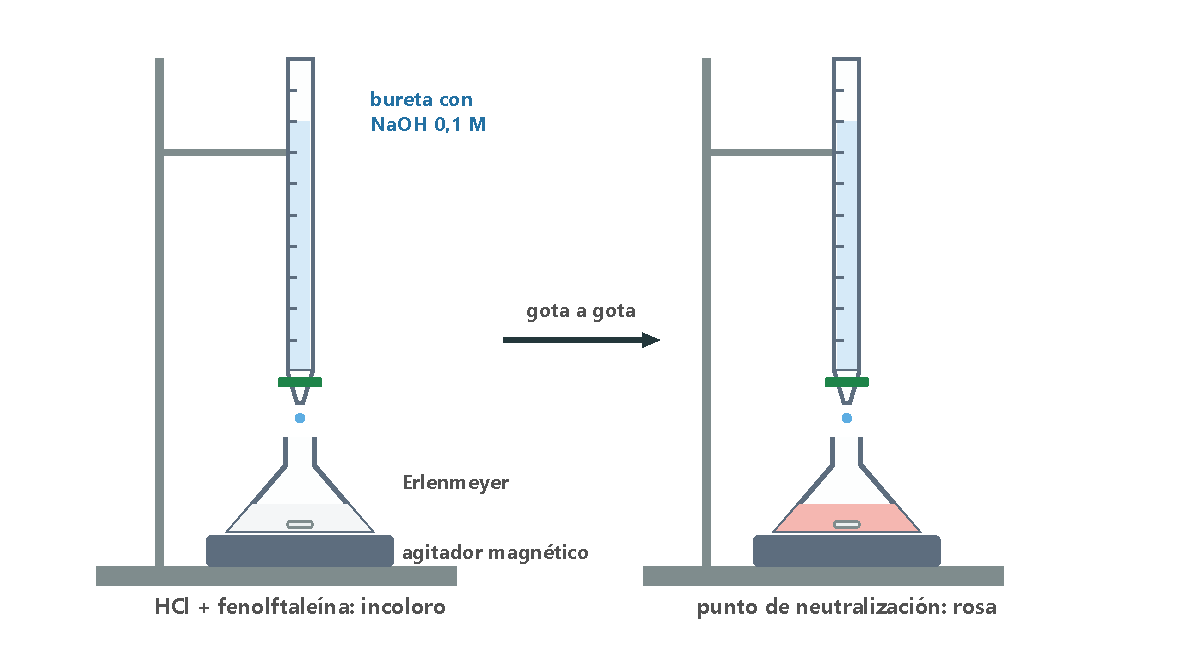
\includegraphics[width=0.75\textwidth]{images/UD6/valoracion}
    \caption{Valoración de un ácido con una base.}
    \label{fig:valoracion}
\end{figure}

\begin{exercise}
    Responde a estas preguntas sobre la práctica:
    \begin{enumerate}[label=\alph*)]
        \item ¿De qué color está la fenolftaleína en la disolución de \ch{HCl}? ¿Y después de la neutralización?
        \item Escribe la ecuación de la reacción.
        \item ¿Para qué sirve el agitador magnético?
        \item ¿Por qué hay que lavar el electrodo del pH-metro y guardarlo en agua destilada?
        \item Si se gastan \qty{20}{\mL} de \ch{NaOH} \num{0.1} M para neutralizar \qty{25}{\mL} de \ch{HCl}, ¿cuál es la concentración del ácido? (En el punto de neutralización, moles de \ch{NaOH} = moles de \ch{HCl}.)
    \end{enumerate}
    \begin{solu}
        a) \textcolor{red}{Incolora} en el ácido; \textcolor{red}{rosa} cuando se ha neutralizado (en cuanto hay un ligero exceso de base).
        b) \ch{HCl (aq) + NaOH (aq) -> NaCl (aq) + H2O (l)}.
        c) Para \textcolor{red}{mezclar} bien la disolución y que la base reaccione en cuanto cae.
        d) Para \textcolor{red}{no cometer errores} de medida (que no queden restos de otra disolución) y para que el electrodo no se seque y se estropee.
        e) \(n(\ch{NaOH}) = \num{0.1} \cdot \num{0.020} = \qty{0.002}{\mol} = n(\ch{HCl})\); \(M(\ch{HCl}) = \frac{\num{0.002}}{\num{0.025}} = \textcolor{red}{\qty{0.08}{\mol\per\L}}\).
    \end{solu}
\end{exercise}

%========================================================================================
\section{Unidad 7. La experiencia de Galileo}
%========================================================================================
% (sacado del final de UD7_movimientos_rectilineos.tex)

En un MRUA que parte del reposo, el espacio recorrido es proporcional al cuadrado del tiempo: \(s = \frac{1}{2}\, a\, t^2\). Galileo lo comprobó dejando rodar una bola por un carril inclinado y midiendo el tiempo con un \emph{reloj de agua}: el volumen de agua que caía de un depósito mientras la bola recorría el carril. Vamos a repetir su experiencia.

\begin{figure}[H]
    \centering
    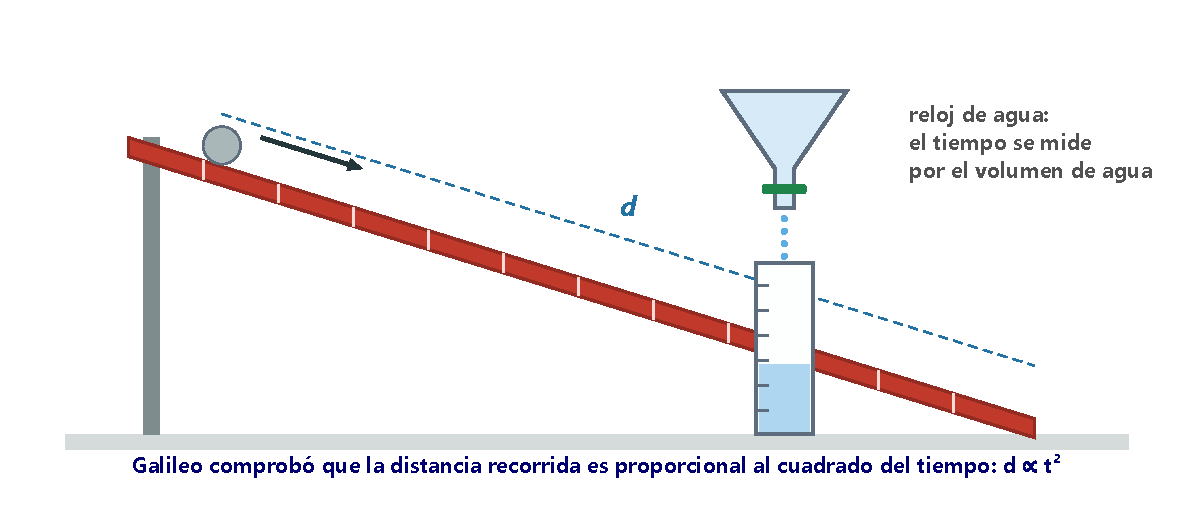
\includegraphics[width=0.75\textwidth]{images/UD7/plano_galileo}
    \caption{Montaje para repetir la experiencia de Galileo.}
    \label{fig:plano_galileo}
\end{figure}

\begin{multicols}{2}
    \textbf{Objetivos}
    \begin{itemize}
        \item Trabajar con materiales del laboratorio de Física y Química.
        \item Respetar las normas de seguridad.
        \item Valorar el trabajo experimental sistemático.
        \item Comprobar la relación entre espacio y tiempo en un MRUA.
    \end{itemize}
    \columnbreak
    \textbf{Material}
    \begin{itemize}
        \item Un carril acanalado de al menos \qty{1}{\m}.
        \item Un embudo con llave y soporte, y una probeta graduada (o un cronómetro).
        \item Una bolita metálica y una cinta métrica.
    \end{itemize}
\end{multicols}

\textbf{Procedimiento}
\begin{enumerate}[label=\numberballgreen]
    \item Fija el carril con una inclinación pequeña y marca la distancia \(d\) entre la bolita y el final del carril.
    \item Llena el embudo de agua y colócalo sobre la probeta.
    \item Suelta la bolita a la vez que abres la llave, y ciérrala cuando la bolita llegue al final. El tiempo se mide en mL de agua (o con el cronómetro).
    \item Repite la experiencia para cuatro distancias distintas (y varias veces cada una).
\end{enumerate}

\begin{exercise}
    Anota tus resultados en una tabla con las columnas \(d\) (m), \(t\) y \(t^2\), compáralos con los del resto de la clase y represéntalos en dos gráficas: \(d\) frente a \(t\) y \(d\) frente a \(t^2\).
    \begin{enumerate}[label=\alph*)]
        \item ¿Qué forma tiene la gráfica \(d\)-\(t\)? ¿Por qué?
        \item ¿Qué relación encuentras entre \(d\) y \(t^2\)?
    \end{enumerate}
    \begin{solu}
        Respuesta según los datos del laboratorio. a) La gráfica \(d\)-\(t\) es una \textcolor{red}{parábola} (curva), porque en un MRUA el espacio no es proporcional al tiempo. b) La gráfica \(d\)-\(t^2\) es una \textcolor{red}{recta que pasa por el origen}: \(d\) es \textcolor{red}{directamente proporcional a \(t^2\)}, y la pendiente vale \(\frac{a}{2}\).
    \end{solu}
\end{exercise}

%========================================================================================
\section{Unidad 8. Factores que afectan a la fuerza de rozamiento}
%========================================================================================
% (sacado del final de UD8_fuerzas.tex)

Vamos a hacer unos experimentos sencillos para averiguar de qué depende la fuerza de rozamiento entre dos cuerpos, con el montaje de la figura~\ref{fig:rozamiento_montaje}.

\begin{multicols}{2}
    \textbf{Objetivos}
    \begin{itemize}
        \item Trabajar con materiales e instrumentos del laboratorio de Física.
        \item Respetar las normas de seguridad.
        \item Valorar el trabajo experimental sistemático.
        \item Comprobar algunos factores de los que depende la fuerza de rozamiento.
    \end{itemize}
    \columnbreak
    \textbf{Material}
    \begin{itemize}
        \item Un sistema de polea y portapesas.
        \item Un bloque de madera de masa conocida y otro de plástico de la misma masa.
        \item Varias pesas de \qty{0.1}{\kg} a \qty{0.5}{\kg}.
        \item Un dinamómetro (puede sustituir al portapesas).
    \end{itemize}
\end{multicols}

\textbf{Procedimiento}
\begin{enumerate}[label=\numberballgreen]
    \item Monta el sistema y añade poco a poco pesas al portapesas (o tira con el dinamómetro) hasta que el bloque de madera empiece a deslizar. Anota el peso del portapesas.
    \item Coloca una pesa de \qty{0.1}{\kg} sobre el bloque y repite la medida. Repítelo con dos y con tres pesas.
    \item Apoya el bloque sobre otra de sus caras (de distinta área) y repite la medida.
    \item Repite el paso 1 con el bloque de plástico.
\end{enumerate}

\begin{exercise}
    Responde a estas preguntas sobre la práctica:
    \begin{enumerate}[label=\alph*)]
        \item ¿Cómo mides la fuerza de rozamiento entre el bloque y la mesa?
        \item Anota en una tabla el peso del bloque (con 0, 1, 2 y 3 pesas) y la fuerza de rozamiento. ¿Qué relación encuentras?
        \item ¿Cambia la fuerza de rozamiento al apoyar el bloque sobre otra cara?
        \item ¿Cómo influye la naturaleza de las superficies (madera o plástico)?
    \end{enumerate}
    \begin{solu}
        Respuesta según los datos del laboratorio. Lo esperable es:
        a) Cuando el bloque empieza a moverse, la fuerza aplicada \textcolor{red}{iguala} a la de rozamiento: esta es el peso del portapesas (o lo que marca el dinamómetro).
        b) La fuerza de rozamiento es \textcolor{red}{proporcional al peso} del bloque (a la normal): al duplicar el peso, se duplica. El cociente \(F_\text{roz}/N\) es el coeficiente de rozamiento.
        c) \textcolor{red}{No}: no depende del área de contacto.
        d) Con superficies distintas el rozamiento es \textcolor{red}{distinto}: depende de la naturaleza de las superficies (normalmente el plástico liso roza menos que la madera).
    \end{solu}
\end{exercise}

%========================================================================================
\section[Unidad 9. La gravedad con un péndulo]{Unidad 9. Cálculo de la gravedad con un péndulo simple}
%========================================================================================
% (sacado del final de UD9_movimiento_circular.tex)

Un \textbf{péndulo simple} es una bolita pesada colgada de un hilo que puede oscilar libremente alrededor de su posición de equilibrio. Si las oscilaciones son pequeñas, el tiempo que tarda en ir y volver (su período) solo depende de la longitud del hilo, \(L\), y de la gravedad, \(g\):
\[ T = 2\pi \sqrt{\frac{L}{g}} \qquad\Rightarrow\qquad g = \frac{4\pi^2 \cdot L}{T^2} \]
Midiendo \(L\) y \(T\) podemos calcular \(g\) en el laboratorio.

\begin{figure}[H]
    \centering
    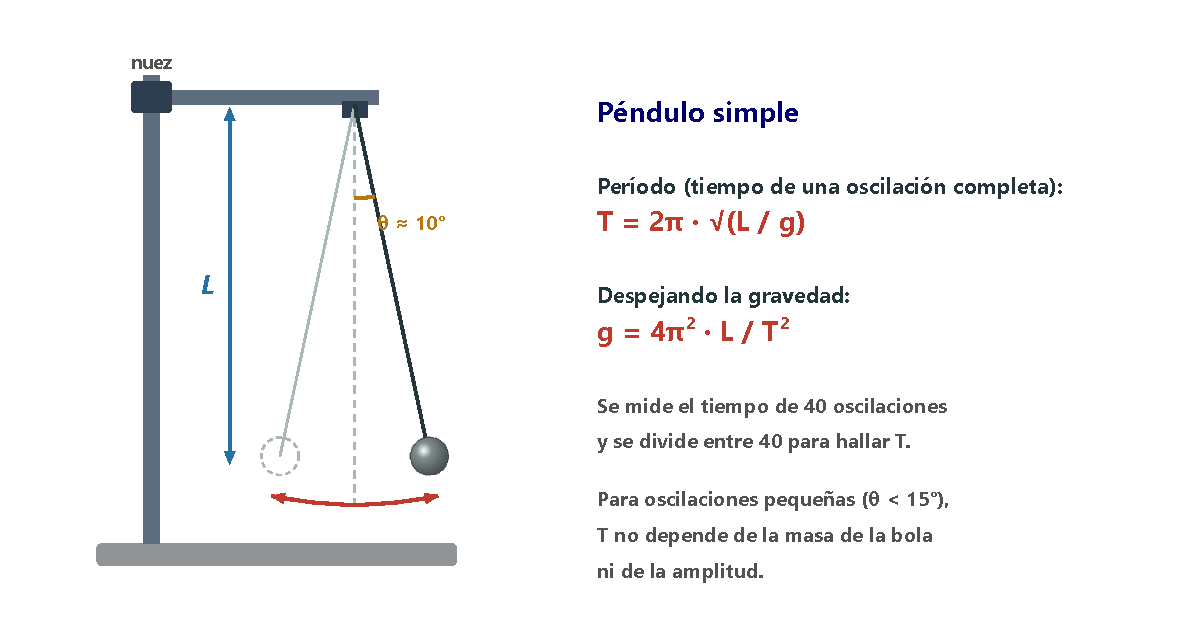
\includegraphics[width=0.8\textwidth]{images/UD9/pendulo}
    \caption{Montaje del péndulo simple.}
    \label{fig:pendulo}
\end{figure}

\noindent\begin{minipage}{\textwidth}
\begin{multicols}{2}
    \textbf{Objetivos}
    \begin{itemize}
        \item Trabajar con materiales e instrumentos del laboratorio de Física.
        \item Valorar el trabajo experimental sistemático.
        \item Medir longitudes y tiempos con los instrumentos adecuados.
        \item Calcular la aceleración de la gravedad a partir de medidas indirectas.
    \end{itemize}
    \columnbreak
    \textbf{Material}
    \begin{itemize}
        \item Un soporte con una pinza metálica y una nuez.
        \item Un hilo de longitud \(L\) (por ejemplo, \qty{1}{\m}) y una cinta métrica.
        \item Una bolita pesada (mejor metálica) con enganche.
        \item Un cronómetro y un transportador de ángulos.
    \end{itemize}
\end{multicols}
\end{minipage}

\textbf{Procedimiento}
\begin{enumerate}[label=\numberballgreen]
    \item Monta el péndulo como en la figura~\ref{fig:pendulo}. Mide la longitud \(L\) desde el punto de suspensión hasta el centro de la bolita.
    \item Separa la bolita unos \ang{10} de la posición de equilibrio y suéltala sin empujarla. Las oscilaciones no deben ser muy abiertas.
    \item Cronometra el tiempo de 40 oscilaciones completas y divídelo entre 40 para obtener el período. Repite la medida al menos cinco veces.
\end{enumerate}

\begin{exercise}
    Responde a estas preguntas sobre la práctica:
    \begin{enumerate}[label=\alph*)]
        \item Anota en una tabla, para cada medida, el tiempo de 40 oscilaciones, el período y el valor de \(g\). ¿Por qué medimos 40 oscilaciones en lugar de una sola?
        \item Calcula la media de los valores de \(g\) y compárala con \qty{9.8}{\m\per\square\s}.
        \item ¿En qué pasos del experimento se cometen más errores de medida?
        \item Con un hilo de \qty{1.00}{\m}, un grupo mide \qty{80.4}{\s} para 40 oscilaciones. ¿Qué valor de \(g\) obtiene?
    \end{enumerate}
    \begin{solu}
        a) Respuesta según los datos. Medir 40 oscilaciones es \textcolor{red}{más fácil y más preciso}: el error al poner en marcha y parar el cronómetro (unas décimas de segundo) se reparte entre las 40 oscilaciones.
        b) Respuesta libre; el resultado suele estar cerca de \qty{9.8}{\m\per\square\s}, aunque los errores de medida pueden ser importantes.
        c) Al \textcolor{red}{medir la longitud del hilo} (hay que llegar hasta el centro de la bola) y al \textcolor{red}{medir el tiempo} (tiempo de reacción).
        d) \(T = \dfrac{\num{80.4}}{40} = \qty{2.01}{\s}\); \(g = \dfrac{4\pi^2 \cdot \num{1.00}}{\num{2.01}^2} = \textcolor{red}{\qty{9.77}{\m\per\square\s}}\).
    \end{solu}
\end{exercise}

%========================================================================================
\section[Unidad 10. Principio de Arquímedes]{Unidad 10. Comprobación del principio de Arquímedes}
%========================================================================================
% (sacado del final de UD10_fluidos.tex)

Vamos a comprobar que un cuerpo sumergido en agua recibe un empuje igual al peso del agua que desaloja:
\[ \text{Empuje} = \text{peso en el aire} - \text{peso en el agua} = \text{peso del agua desalojada} \]


\noindent\begin{minipage}[t]{0.53\textwidth}
    \textbf{Objetivos}
    \begin{itemize}
        \item Trabajar con materiales e instrumentos del laboratorio de Física.
        \item Valorar el trabajo experimental sistemático, evitando errores de paralaje.
        \item Comprobar la relación entre el empuje, el peso en el aire y el peso en el agua de un cuerpo.
        \item Calcular la densidad de un cuerpo.
    \end{itemize}
\end{minipage}\hfill
\begin{minipage}[t]{0.43\textwidth}
    \textbf{Material}
    \begin{itemize}
        \item Un soporte con una pinza metálica y una nuez.
        \item Un dinamómetro y una probeta graduada.
        \item Una esfera de metal con enganche e hilo.
        \item Agua.
    \end{itemize}
\end{minipage}

\medskip

\textbf{Procedimiento} (el montaje es como el de la figura~\ref{fig:empuje})
\begin{enumerate}[label=\numberballgreen]
    \item Cuelga la esfera del dinamómetro y anota su peso en el aire.
    \item Echa agua en la probeta, hasta la mitad aproximadamente, y mide su volumen con cuidado: mira la escala con los ojos a la altura de la superficie del agua para no cometer \textbf{error de paralaje}.
    \item Sumerge la esfera, colgada del dinamómetro, en el agua de la probeta, de modo que quede totalmente cubierta pero sin tocar el fondo. Anota su peso y el nuevo nivel del agua.
    \item Repite el procedimiento tres veces y anota los resultados en una tabla como esta:
\end{enumerate}

\begin{center}
    % --- tabla antigua ---
    % \begin{tblr}{width=\linewidth, colspec={Q[c,m] X[c,m] X[c,m] X[c,m] X[c,m] X[c,m]}, hlines, vlines, row{1}={bg=ocre!85, fg=white, font=\bfseries\small}, cells={font=\small}}
        % Exp. & Peso en el aire (N) & Peso en el agua (N) & Empuje (N) & Volumen inicial (\unit{\cubic\cm}) & Volumen final (\unit{\cubic\cm}) \\
        % 1 & \ldots & \ldots & \ldots & \ldots & \ldots \\
        % 2 & \ldots & \ldots & \ldots & \ldots & \ldots \\
        % 3 & \ldots & \ldots & \ldots & \ldots & \ldots \\
    % \end{tblr}
    % --- tabla nueva ---
    {\small
    \begin{tabular}{@{}c c c c C{0.15\linewidth} C{0.15\linewidth}@{}}
        \toprule
        \textbf{Exp.} & \textbf{Peso en el aire (N)} & \textbf{Peso en el agua (N)} & \textbf{Empuje (N)} & \textbf{Volumen inicial (\unit{\cubic\cm})} & \textbf{Volumen final (\unit{\cubic\cm})} \\
        \midrule
        1 & \ldots & \ldots & \ldots & \ldots & \ldots \\[3pt]
        2 & \ldots & \ldots & \ldots & \ldots & \ldots \\[3pt]
        3 & \ldots & \ldots & \ldots & \ldots & \ldots \\
        \bottomrule
    \end{tabular}
    }
\end{center}

\begin{exercise}
    Responde a estas preguntas sobre la práctica:
    \begin{enumerate}[label=\alph*)]
        \item ¿Cuándo pesa más la esfera, antes o después de sumergirla? Calcula el empuje con los valores medios.
        \item Calcula el volumen de agua desalojada (aumento de volumen en la probeta). ¿Qué relación tiene con el volumen de la esfera?
        \item Calcula el peso del agua desalojada y compáralo con el empuje.
        \item Calcula la densidad de la esfera.
        \item ¿Qué empuje recibiría la esfera en alcohol (\qty{790}{\kg\per\cubic\m})?
        \item Un grupo obtiene estos valores medios: peso en el aire, \qty{2.40}{\newton}; peso en el agua, \qty{2.09}{\newton}; el nivel sube de \qty{50}{\cubic\cm} a \qty{82}{\cubic\cm}. Resuelve con ellos los apartados a), c), d) y e).
    \end{enumerate}
    \begin{solu}
        a) Pesa más \textcolor{red}{antes de sumergirla}: el empuje es \(E = P - P_a\).
        b) El volumen desalojado es \textcolor{red}{igual al volumen de la esfera}, porque está totalmente sumergida.
        c) Según el principio de Arquímedes, los dos valores deben coincidir (salvo errores de medida): \(E = V \cdot \rho_{\text{agua}} \cdot g\).
        d) \(\rho = \dfrac{P}{g \cdot V}\).
        e) Sería \textcolor{red}{menor}, porque el alcohol es menos denso que el agua.
        f) \(E = \num{2.40} - \num{2.09} = \textcolor{red}{\qty{0.31}{\newton}}\). \(V = 82 - 50 = \qty{32}{\cubic\cm}\); peso del agua desalojada: \(\num{32e-6} \cdot 1000 \cdot \num{9.8} = \textcolor{red}{\qty{0.31}{\newton}}\), igual al empuje.
        \(\rho = \dfrac{\num{2.40}}{\num{9.8} \cdot \num{32e-6}} = \textcolor{red}{\qty{7650}{\kg\per\cubic\m}}\) (parece acero). En alcohol: \(E = \num{32e-6} \cdot 790 \cdot \num{9.8} = \textcolor{red}{\qty{0.25}{\newton}}\).
    \end{solu}
\end{exercise}

%========================================================================================
\section[Unidad 11. Conservación de la energía]{Unidad 11. Comprobación del principio de conservación de la energía}
%========================================================================================
% (sacado del final de UD11_energia.tex)

Con un péndulo simple, como el de la práctica de la unidad anterior, podemos comprobar que la energía mecánica se conserva: la energía potencial de la bola en la posición inicial se transforma en energía cinética en el punto más bajo, y otra vez en potencial al subir por el otro lado.

\begin{figure}[H]
    \centering
    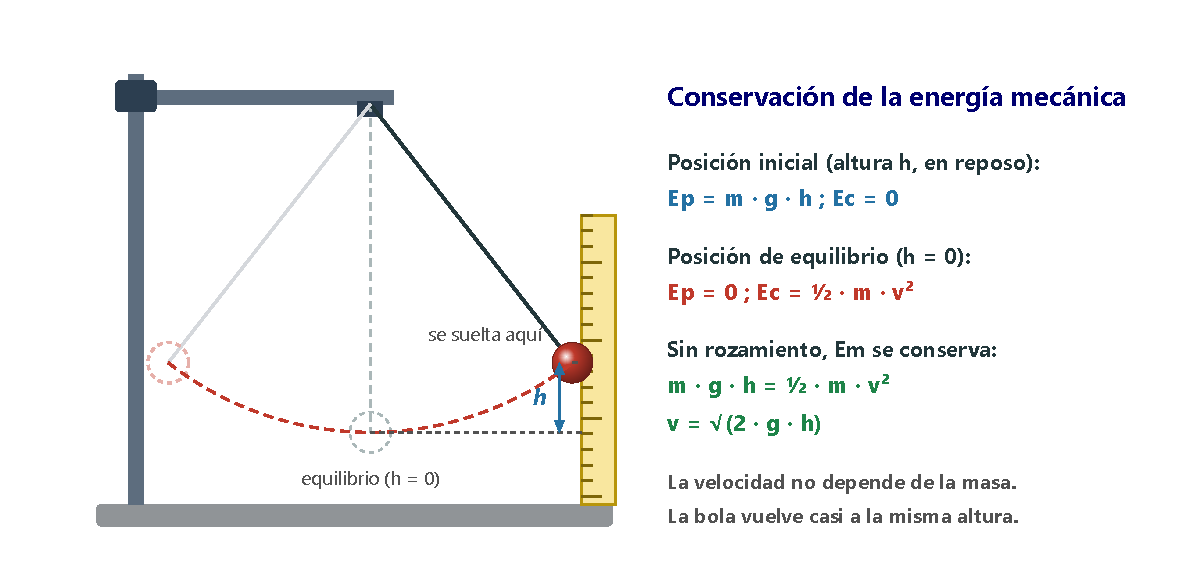
\includegraphics[width=0.9\textwidth]{images/UD11/pendulo_energia}
    \caption{Montaje del péndulo para comprobar la conservación de la energía mecánica.}
    \label{fig:pendulo_energia}
\end{figure}

\noindent\begin{minipage}[t]{0.53\textwidth}
    \textbf{Objetivos}
    \begin{itemize}
        \item Trabajar con materiales e instrumentos del laboratorio de Física.
        \item Valorar el trabajo experimental sistemático.
        \item Medir longitudes con los instrumentos adecuados.
        \item Comprobar el principio de conservación de la energía mecánica.
    \end{itemize}
\end{minipage}\hfill
\begin{minipage}[t]{0.43\textwidth}
    \textbf{Material}
    \begin{itemize}
        \item Un soporte con una pinza metálica y una nuez.
        \item Una esfera de metal y un hilo.
        \item Una regla.
    \end{itemize}
\end{minipage}

\medskip

\textbf{Procedimiento}
\begin{enumerate}[label=\numberballgreen]
    \item Monta el péndulo como en la figura~\ref{fig:pendulo_energia} y sujeta la bola al extremo del hilo.
    \item Coloca la regla en vertical, con el cero (\(h = 0\)) a la altura de la bola en la posición de equilibrio.
    \item Separa la bola hasta que esté a una altura \(h\) que puedas medir con la regla y suéltala sin empujarla.
    \item Observa si, después de una oscilación completa, la bola vuelve a la misma altura.
\end{enumerate}

\begin{exercise}
    Responde a estas preguntas sobre la práctica:
    \begin{enumerate}[label=\alph*)]
        \item ¿Qué tipo de energía tiene la bola en la posición inicial, a la altura \(h\)? ¿Y al pasar por la posición de equilibrio? Explica con un esquema las transformaciones de energía.
        \item Demuestra que la velocidad de la bola en la posición de equilibrio es \(v = \sqrt{2 \cdot g \cdot h}\). ¿Hace falta conocer su masa?
        \item ¿Con qué velocidad pasa por la posición de equilibrio si se suelta desde \qty{20}{\cm}?
        \item Si la bola tiene \qty{25}{\gram}, completa la tabla en tu cuaderno:
        \begin{center}
            % --- tabla antigua ---
            % \begin{tblr}{colspec={cccc}, hlines, vlines, row{1}={bg=ocre!85, fg=white, font=\bfseries\small}, cells={font=\small}}
                % \(h\) (cm) & \(E_p\) inicial (J) & \(E_c\) en el equilibrio (J) & \(v\) en el equilibrio (m/s) \\
                % 15 & \ldots & \ldots & \ldots \\
                % 20 & \ldots & \ldots & \ldots \\
                % 25 & \ldots & \ldots & \ldots \\
                % 30 & \ldots & \ldots & \ldots \\
            % \end{tblr}
            % --- tabla nueva ---
            {\small
            \begin{tabular}{@{}cccc@{}}
                \toprule
                \textbf{\(h\) (cm)} & \textbf{\(E_p\) inicial (J)} & \textbf{\(E_c\) en el equilibrio (J)} & \textbf{\(v\) en el equilibrio (m/s)} \\
                \midrule
                15 & \ldots & \ldots & \ldots \\[3pt]
                20 & \ldots & \ldots & \ldots \\[3pt]
                25 & \ldots & \ldots & \ldots \\[3pt]
                30 & \ldots & \ldots & \ldots \\
                \bottomrule
            \end{tabular}
            }
        \end{center}
        \item ¿Vuelve la bola exactamente a la misma altura? ¿Por qué?
    \end{enumerate}
    \begin{solu}
        a) Al principio, solo \textcolor{red}{energía potencial}; en la posición de equilibrio, solo \textcolor{red}{energía cinética}. Mientras baja, la potencial se transforma en cinética, y al subir por el otro lado ocurre al revés.
        b) \(m \cdot g \cdot h = \frac{1}{2} \cdot m \cdot v^2 \Rightarrow v = \sqrt{2 \cdot g \cdot h}\): la masa se simplifica, así que \textcolor{red}{no hace falta conocerla}.
        c) \(v = \sqrt{2 \cdot \num{9.8} \cdot \num{0.20}} = \textcolor{red}{\qty{1.98}{\m\per\s}}\).
        d) Con \(E_p = \num{0.025} \cdot \num{9.8} \cdot h\) y \(E_c = E_p\): \qty{15}{\cm}: \qty{0.037}{\joule}, \qty{1.71}{\m\per\s}; \qty{20}{\cm}: \qty{0.049}{\joule}, \qty{1.98}{\m\per\s}; \qty{25}{\cm}: \qty{0.061}{\joule}, \qty{2.21}{\m\per\s}; \qty{30}{\cm}: \qty{0.074}{\joule}, \qty{2.42}{\m\per\s}.
        e) Llega \textcolor{red}{casi} a la misma altura, pero un poco más abajo: el \textcolor{red}{rozamiento con el aire} transforma una pequeña parte de la energía mecánica en térmica, y tras muchas oscilaciones el péndulo se para.
    \end{solu}
\end{exercise}

%========================================================================================
\section[Unidad 12. Calor específico]{Unidad 12. Medida de la capacidad calorífica específica}
%========================================================================================
% (sacado del final de UD12_calor.tex)

La capacidad calorífica específica es una propiedad característica: sustancias distintas suben su temperatura de forma diferente cuando reciben la misma cantidad de calor. En esta práctica la mediremos con un calorímetro, aplicando el balance de energía:
\[ m_1 \cdot c_1 \cdot (T_1 - T_{\text{eq}}) = m_2 \cdot c_2 \cdot (T_{\text{eq}} - T_2) \]

\begin{figure}[H]
    \centering
    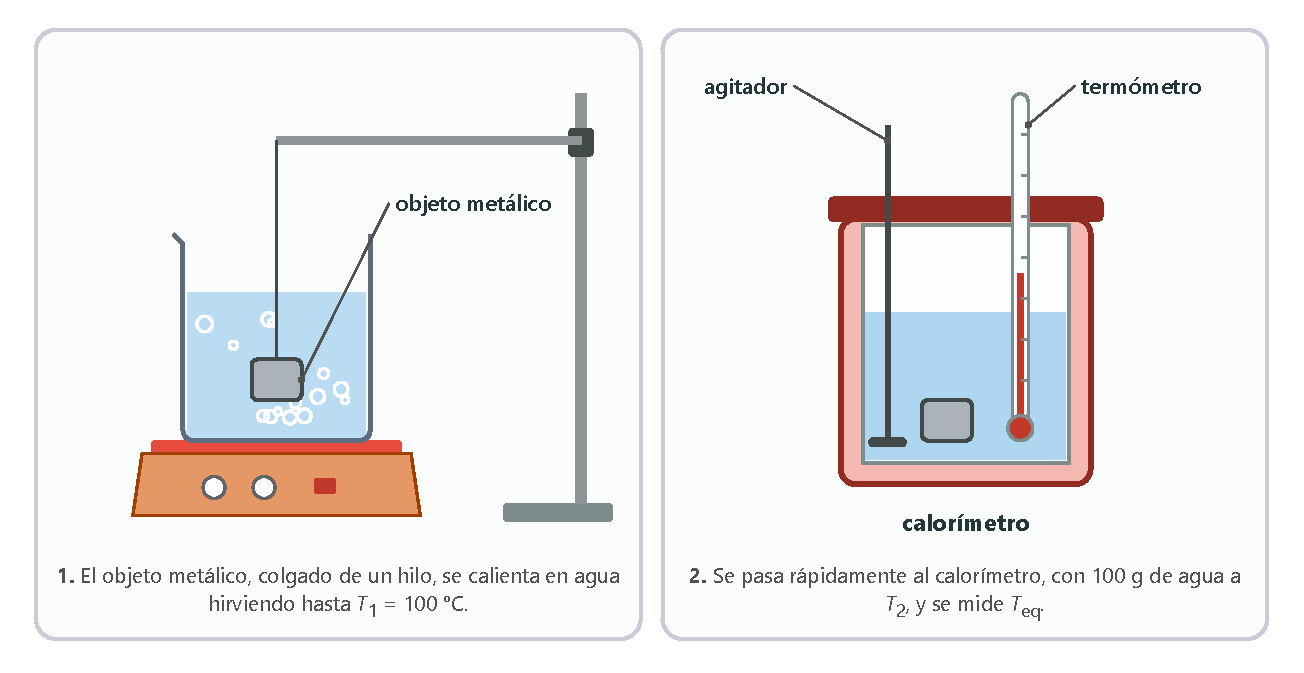
\includegraphics[width=\textwidth]{images/UD12/practica_calor_especifico}
    \caption{Montaje para medir la capacidad calorífica específica de un metal.}
    \label{fig:practica_calor_especifico}
\end{figure}

\noindent\begin{minipage}[t]{0.53\textwidth}
    \textbf{Objetivos}
    \begin{itemize}
        \item Trabajar con materiales e instrumentos del laboratorio de Física.
        \item Valorar el trabajo experimental sistemático.
        \item Medir masas y temperaturas con los instrumentos adecuados.
        \item Medir la capacidad calorífica específica de un objeto metálico.
    \end{itemize}
\end{minipage}\hfill
\begin{minipage}[t]{0.43\textwidth}
    \textbf{Material}
    \begin{itemize}
        \item Un vaso de precipitados y un hornillo.
        \item Un calorímetro y un termómetro.
        \item \qty{100}{\gram} de agua.
        \item Un objeto metálico de masa conocida y un hilo.
        \item Un soporte con pinza.
    \end{itemize}
\end{minipage}

\medskip

\textbf{Procedimiento}
\begin{enumerate}[label=\numberballgreen]
    \item Ata el objeto metálico a un hilo y sumérgelo en un vaso de precipitados con agua. Calienta hasta que el agua hierva: el objeto estará a la temperatura de ebullición, \(T_1\).
    \item Mientras el agua hierve, echa en el calorímetro \qty{100}{\gram} de agua a temperatura ambiente. Tápalo, introduce el termómetro, espera unos minutos y anota su temperatura, \(T_2\).
    \item Cuando el agua del vaso lleve un rato hirviendo, saca el objeto tirando del hilo e introdúcelo rápidamente en el calorímetro. Tápalo y agita suavemente con la varilla.
    \item Anota la temperatura máxima que marca el termómetro: es la temperatura de equilibrio, \(T_{\text{eq}}\).
    \item Repite el experimento varias veces y calcula el valor medio de \(T_{\text{eq}}\).
\end{enumerate}

\begin{exercise}
    Un grupo de alumnos ha usado un objeto metálico de \qty{80}{\gram} y \qty{100}{\gram} de agua a \(T_2 = \qty{20.0}{\degreeCelsius}\). Estas son sus medidas:
    \begin{center}
        % --- tabla antigua ---
        % \begin{tblr}{colspec={cccccc}, hlines, vlines, row{1}={bg=ocre!85, fg=white, font=\bfseries}}
            % Experiencia & 1 & 2 & 3 & 4 & 5 \\
            % \(T_{\text{eq}}\) (\unit{\degreeCelsius}) & \num{31.6} & \num{32.1} & \num{31.8} & \num{31.5} & \num{32.0} \\
        % \end{tblr}
        % --- tabla nueva ---
        \begin{tabular}{@{}cccccc@{}}
            \toprule
            \textbf{Experiencia} & \textbf{1} & \textbf{2} & \textbf{3} & \textbf{4} & \textbf{5} \\
            \midrule
            \(T_{\text{eq}}\) (\unit{\degreeCelsius}) & \num{31.6} & \num{32.1} & \num{31.8} & \num{31.5} & \num{32.0} \\
            \bottomrule
        \end{tabular}
    \end{center}
    \begin{enumerate}[label=\alph*)]
        \item ¿Qué temperatura, \(T_1\), tiene el objeto cuando lo sacas del vaso?
        \item Calcula el valor medio de la temperatura de equilibrio.
        \item Calcula la capacidad calorífica específica del metal.
        \item ¿De qué metal puede estar hecho el objeto? ¿Por qué el resultado no coincide exactamente con el de la tabla?
    \end{enumerate}
    \begin{solu}
        a) Ha alcanzado el equilibrio térmico con el agua hirviendo, así que está a \textcolor{red}{\qty{100}{\degreeCelsius}} (aproximadamente; depende de la presión atmosférica).
        b) \(T_{\text{eq}} = \dfrac{\num{31.6} + \num{32.1} + \num{31.8} + \num{31.5} + \num{32.0}}{5} = \textcolor{red}{\qty{31.8}{\degreeCelsius}}\).
        c) \(\num{0.080} \cdot c \cdot (100 - \num{31.8}) = \num{0.100} \cdot 4180 \cdot (\num{31.8} - \num{20.0}) \Rightarrow \num{5.456} \cdot c = \num{4932.4}\)
        \[ c = \textcolor{red}{\qty{904}{\cunit}} \]
        d) Probablemente es \textcolor{red}{aluminio} (\qty{910}{\cunit}). La diferencia se debe a los errores de medida, a la energía que se pierde al trasladar el objeto y a que no hemos tenido en cuenta el calor que absorbe el propio calorímetro.
    \end{solu}
\end{exercise}

%========================================================================================
\section{Unidad 13. La resonancia acústica}
%========================================================================================
% (sacado del final de UD13_luz_sonido.tex)

Todos los objetos, y también las columnas de aire encerradas en un tubo, tienen una o varias \textbf{frecuencias naturales} de vibración. Si les llega una onda que vibra justo con una de esas frecuencias, empiezan a vibrar con una amplitud cada vez mayor y el sonido se refuerza. Este fenómeno se llama \textbf{resonancia}.

\begin{figure}[H]
    \centering
    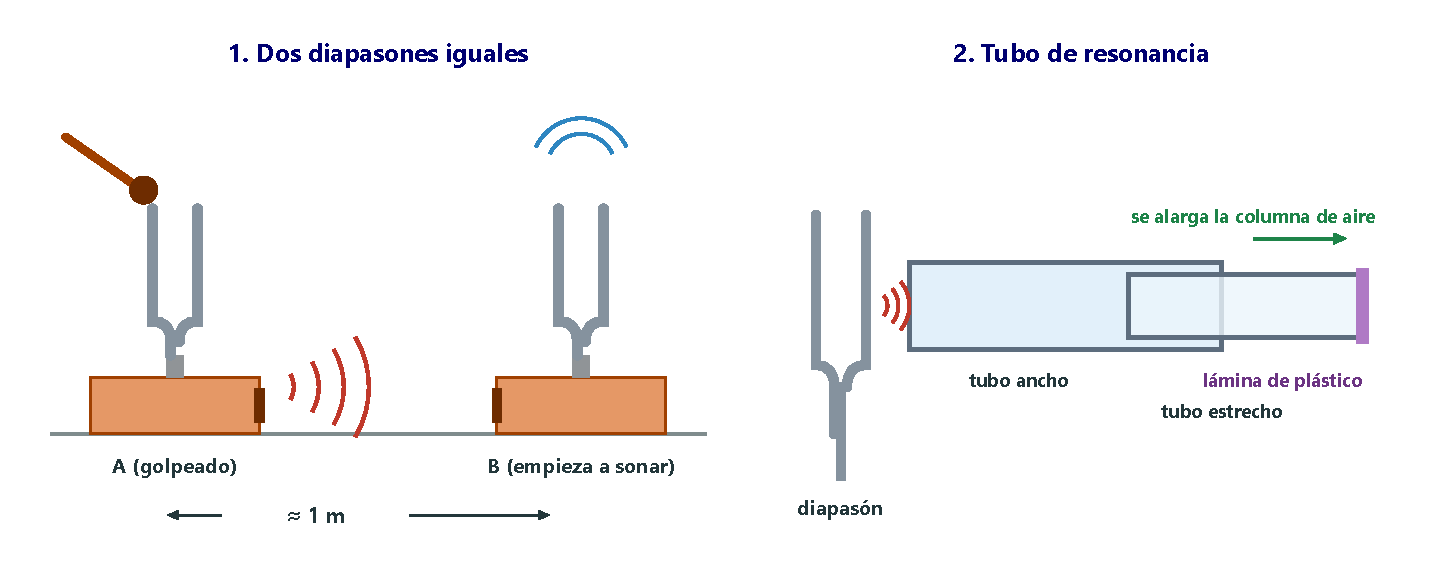
\includegraphics[width=\textwidth]{images/UD13/practica_resonancia}
    \caption{Montajes de la práctica: dos diapasones iguales enfrentados (1) y un tubo de resonancia de longitud variable (2).}
    \label{fig:practica_resonancia}
\end{figure}

\noindent\begin{minipage}[t]{0.53\textwidth}
    \textbf{Objetivos}
    \begin{itemize}
        \item Comprobar experimentalmente la resonancia acústica en un tubo.
        \item Comprobar que un diapasón hace vibrar por resonancia a otro igual.
        \item Trabajar con materiales del laboratorio de Física.
        \item Valorar la importancia del trabajo experimental.
    \end{itemize}
\end{minipage}\hfill
\begin{minipage}[t]{0.43\textwidth}
    \textbf{Material}
    \begin{itemize}
        \item Dos tubos de plástico rígido que encajen uno dentro del otro.
        \item Dos diapasones de la misma frecuencia con caja de resonancia.
        \item Un martillo de goma y una regla.
        \item Una lámina de plástico.
    \end{itemize}
\end{minipage}

\medskip

\textbf{Procedimiento}
\begin{enumerate}[label=\numberballgreen]
    \item Coloca los dos diapasones a \qty{1}{\m} de distancia, con las aberturas de sus cajas enfrentadas. Golpea uno con el martillo de goma y escucha. Al cabo de unos segundos, tócalo con los dedos para que deje de sonar.
    \item Coge el otro diapasón por la parte trasera de su caja y acércalo al oído: oirás que está sonando, aunque nadie lo ha golpeado. La vibración ha pasado de un diapasón a otro por resonancia.
    \item Introduce el tubo estrecho en el ancho y tapa con la lámina de plástico el extremo libre del tubo estrecho. Golpea un diapasón (sin caja) y colócalo delante de la boca del tubo ancho.
    \item Sin dejar de escuchar, desliza el tubo estrecho hacia fuera para alargar la columna de aire. Anota con la regla la longitud para la que el sonido se oye con más fuerza. Repite la experiencia varias veces.
\end{enumerate}

\begin{exercise}
    Explica cómo se transmite el sonido de un diapasón al otro.
    \begin{solu}
        El diapasón golpeado hace vibrar el aire, y la onda sonora llega al segundo diapasón. Como los dos tienen la \textcolor{red}{misma frecuencia natural}, el segundo empieza a vibrar cada vez con más amplitud: es la \textcolor{red}{resonancia}.
    \end{solu}
\end{exercise}

\begin{exercise}
    A partir de la experiencia, responde:
    \begin{enumerate}[label=\alph*)]
        \item ¿Habrías conseguido el mismo efecto con dos diapasones de distinta frecuencia?
        \item ¿Crees que la resonancia en tubos está relacionada con el sonido de algunos instrumentos musicales?
        \item ¿Qué relación puede haber entre la longitud del tubo y que el sonido sea más agudo o más grave?
    \end{enumerate}
    \begin{solu}
        a) \textcolor{red}{No}: solo hay resonancia si la frecuencia de la onda coincide con la frecuencia natural del segundo diapasón.
        b) \textcolor{red}{Sí}: en los instrumentos de viento (flauta, clarinete, trompeta, órgano) la columna de aire del tubo resuena y refuerza ciertas notas; en los de cuerda, la caja de resonancia amplifica el sonido de las cuerdas.
        c) Cuanto \textcolor{red}{más largo es el tubo, más grave} es el sonido con el que resuena (menor frecuencia); los tubos cortos resuenan con sonidos agudos. Por eso los tubos de un órgano son de distintas longitudes.
    \end{solu}
\end{exercise}

\begin{exercise}
    En un tubo cerrado por un extremo, el primer refuerzo del sonido se produce cuando la longitud de la columna de aire es la cuarta parte de la longitud de onda, \(L = \lambda/4\). Un grupo usa un diapasón de \qty{440}{\hertz} y oye el primer refuerzo con \(L = \qty{19.5}{\cm}\). Calcula la velocidad del sonido que se deduce de su medida.
    \begin{solu}
        \(\lambda = 4L = 4 \cdot \num{0.195} = \qty{0.78}{\m}\). \(v = \lambda \cdot f = \num{0.78} \cdot 440 = \textcolor{red}{\qty{343}{\m\per\s}}\), muy próxima al valor tabulado (\(\approx \qty{340}{\m\per\s}\)).
    \end{solu}
\end{exercise}
